% !TeX root = ../main.tex
% Add the above to each chapter to make compiling the PDF easier in some editors.

\chapter{Theoretical Background}\label{chapter:theoreticalBackground}
Spiking Neural Networks (SNNs) try to mimic the functional mechanisms of brains. This can give a better understanding on how brains work and learn, as well as the option to build artificial brains in form of SNNs and use them to solve tasks. The complexity of these Artificial Neural Networks (ANN) is capped by the available computation time or specialised hardware as well as the understanding of how to structure the network and set it’s parameters. To get a complete picture of the ideas and mechanisms that are enabling a SNN to learn how to solve tasks, this chapter gives an introduction to basic mechanisms in biological brains and an overview about the evolution of Artificial Neural Networks.
\section{Biological Background}
The knowledge about the structure and understanding of what enables brains to perform complex tasks is still incomplete. As result of lacking methods and instruments to examine the structure of brains, only in the late 19th century the neuron as primary functional unit was discoverd. The spansih anatomist Santiago Ramón y Cajal proposed that neurons are, other to former believes, discrete functional units and not connected in a meshwork. This is called the Neuron doctrine and got updated and refined  in the following centuries\cite{10.2307/1757040}. It is the foundation of todays understanding of the brain. The key elements of the doctrine specify that the brain is made up of individual units which are cells and can be specialised. These units are called Neurons and are generated by cell division. They are connected by Synapses and are mainly one directional and can either be excitatory or inhibitory\cite{lopez2006neuron}.
\newline
Todays model of a neuron consists of many different parts necessary to function. These are shown in the schemata in \autoref{fig:neuronShema}.
\begin{figure}[htpb]
  \centering
  \includegraphics[width = \textwidth]{figures/Neuron.png}
  \caption{Overview about the main parts of a Neuron \cite{wikiNeuron}}
  \label{fig:neuronShema}
\end{figure}
The main part of a cell is called soma. It is the  body of a cell and holds the nucleus. Together they are responsible for keeping the cell alive as well as for reproduction, as the nucleus also holds the DNA.
The treelike structure reaching out from the Soma is called Dendrite. The different branches end near the axons of other cells and accept stimuli from them. It also tends to branch out from few main stems, channeling the connection from many other cells. Stimuli from other neurons change the electrical potential of the cell membrane. While the membrane potential degrades slowly over time, receiving enough excitation overcoming the decay, the potential rises to a threshold level and an electrical impulse discharges along the axon to the axon terminals resetting the membrane potential. The axon leads the signal to other neurons and largely varies in length as it may connect to other brain regions. In the area around the end of the axon it again branches out in small axon terminals connecting to the dendrit of different neurons. Human brains are estimated to have 86 billion neurons forming a complex network with their connection.
\newline
As the neurons are separate cells there is a gap between axon terminals and dendrit which is called Synaptic Gap. There are two main types of synapses differentiated by the way the information is passed. One type is based on electric transmission of the signal, the other uses chemicals to travel the gap and stimulate the neuron. The chemical transmission is believed to make up most of the connection and is also the one simulated by the spiking neural networks used for this thesis. In \autoref{fig:chemicalSynaps} the main parts building a chemical synapse are shown.
\begin{figure}[htpb]
  \centering
  \includegraphics[scale=0.25]{figures/synapse.png}
  \caption{Schemata of a Synapse \cite{wikiSyn}}
  \label{fig:chemicalSynaps}
\end{figure}
To transmit an incoming signal the axon terminal releases neurotransmitters to the gap which can be received by the dendrit through receptors. Neurotransmitters are build in the terminal or reabsorbed from the gap. In the terminal they are held in Synaptic Vesicles which can fuse with voltage gated calcium channels releasing the transmitters to the gap\cite{Catterall411}. How good the connection transmits the signal depends mainly on the amount of neurotransmitters released as well as the amount of receptors at the dendrite. 
In the synaptic gap there also can be neuromodulators eg. Dopamine which are believed to change how the synapse evolves over time and thus amplify or diminish changes in the strength of the connection.

\section{Artificial Neural Networks}
To explore how these networks act the neurophysiologist Warren McCulloch and the mathematician Walter Pitts developed the first mathematical model in 1943 \cite{mcculloch1943logical}. This model, known as McCulloch-Pitts-Model is a strongly simplified description of a Neuron and shown in \autoref{fig:MCPShema}. It has binary inputs and a binary output. If the sum over the  inputs exceeds a threshold the output is $1$ otherwise it is $0$. Inventing the Perceptron Frank Rosenblatt proposed 1962 a model overcoming the limitations to boolean inputs and using real-valued weights on the inputs.
\begin{figure}[htpb]
  \centering
  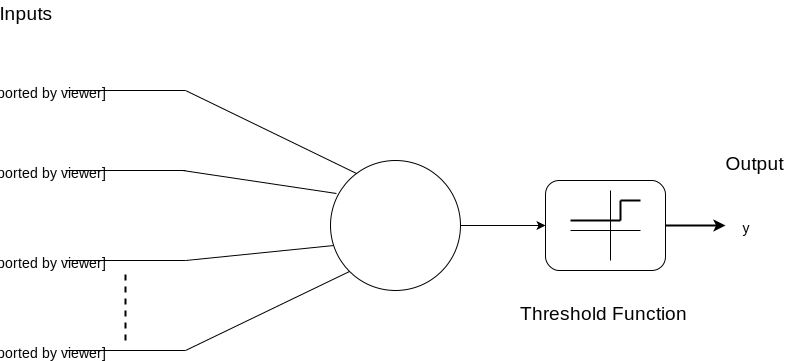
\includegraphics[scale=0.65]{figures/McPSchema.pdf}
  \caption[Schemata of McCulloch-Pitts-Model]{Schemata of a Synapse \cite{wikiSyn}}
  \label{fig:MCPShema}
\end{figure}
\newline
\autoref{eq:MCP} describes the behaviour of the perceptron where x is a real-valued input vector, w the vector of the weights of the same size and b a bias. 
\newline

\begin{equation}\label{eq:MCP}
  f(x) =
    \begin{cases}
      1 & \text{if $w*x+b > 0$,} \\
      0 & \text{otherwise.}
    \end{cases}  
\end{equation}
By choosing the right weights the perceptron can be used as classifier for linear separable data. Further it can be shown that weights can be learned and converge in linear separable training sets \cite{Bishop:998831}. The algorithm calculates the weight change from comparing the result $y_j$ calculated by the neuron from the feature set $x_j$, with the desired result $d_j$ for each training sample $j$. The weight change for every connection is the result of multiplying the error $d-y$ by the learning rate $r$ and the input $x$ of that connection as shown in \autoref{eq:MCP_weight} .
\newline
\begin{equation}\label{eq:MCP_weight}
  w_i(t+1) = w_i(t) +r * (d_j - y_j(t))*x_{ji} \text{ , for all features $0<=i<=n$}
\end{equation}
By iterating over the set of training samples and updating the weights after each step these converge to the correct values to classify the data.
\newline
For this learning rule the bias is described by setting $x_0$ always to $1$ and have the feature set of size n represented by $x_1$ to xn. Doing so $w_0$ acts as bias for the threshold function and gets adjusted in the learning process.

\section{Second generation of ANN}\label{sec:backprop}
To be able to solve non-linear classifiable data sets multiple perceptrons can be chained to form a network. This construct is referred as Multilayer Perceptron (MP) and consists of at least three layers, the input, hidden and output layer. Unlike a single perceptron the activation function of neurons in MPs are sigmoid shaped. Historically most common is the logistic function:
\begin{equation}\label{eq:logisFunc}
  y_i(v_i) = (1 + e^{-v_i})^{-1}
\end{equation}
where $y$ is the output of the $i$-th neuron for the weighted sum $v_i$ of its input connections.
\autoref{fig:logisFunction} shows the shape of this function.

\begin{figure}[htpb]
  \centering
  \includegraphics[width = \textwidth]{figures/logisticFunc.png}
  \caption{Plot of a logistic function}
  \label{fig:logisFunction}
\end{figure}
For learning the weights an algorithm called back-propagation was proposed 1986 by David Everett Rumelhart and others \cite{rumelhart1988learning}. It generalizes the learning function of the single perceptron. It consists of two main steps for each training sample. First the output for the feature set $x$ is calculated, which is also referenced as information forward propagation. The overall error is the sum of the squared difference in output $o$ to the target $t$ in each output node and is described by the following functions:
\begin{equation}\label{eq:backpErr}
  E = \frac{1}{2} \sum_{i=1}^n (t_i-o_i)^2
\end{equation}
The aim of the back-propagation algorithm is to minimize this error. This is realized by propagating the error in each output back through the network and changing the weights of each connection which is the second step and referred as error back propagation. In this step for each connection the partial derivative of the error with respect to its weight is calculated which describes the impact a change of this weight has on the error and in which direction it changes the error. For each connection this depends on the impact it has on the result oj of the node it connects to and its impact on the error.
\newline
This can formally be described by the first step in this equation:
\begin{equation}\label{eq:backpMainDevi}
  \frac{\partial E}{\partial w_{ij}} =
  \frac{\partial E}{\partial o_j} \frac{\partial o_j}{\partial w_{ij}} = 
  \frac{\partial E}{\partial o_j} \frac{\partial o_j}{\partial net_j} \frac{\partial net_j}{\partial w_{ij}}
\end{equation}

The impact on the output in $o_j$ is dependent on the weights influence on the activation sum $net_j$ of a node, what is used in the second step. In this last factor only one term in the sum depends on $w_{ij}$ thus its derivat is $o_i$
\begin{equation}\label{eq:backp3s}
  \frac{\partial net_j}{\partial w_{ij}} =  \frac{\partial}{\partial w_{ij}} \left( \sum_{k=1}^n w_{kj} o_{kj} \right) = \frac{\partial}{\partial w_{ij}} w_{ij}o_i = o_i
\end{equation}
The second factor in \autoref{eq:backpMainDevi} is the derivative of the output of a node with respect to its input which is the partial derivative of the used activation function and also the reason backpropagation needs a differentiable activation function.
\newline
For connections to output neurons $o_j$ equals to $y_i$ and the first factor can be rewritten as
\begin{equation}
  \frac{\partial E}{\partial o_j} = \frac{\partial E}{\partial y_j} 
\end{equation}
The derivative for the square error from \autoref{eq:backpErr} again only depending in one sum on $y$ resolves to
\begin{equation}\label{eq:backpResEDev}
  \frac{\partial E}{\partial o_j} = \frac{\partial E}{\partial y_j} =
  \frac{\partial}{\partial y_j} \frac{1}{2}(t-y)^2 = y - t 
\end{equation}
Plugging everything together through substitution, the derivative can be rewritten as 
\begin{equation}
  \frac{\partial E}{\partial w_{ij}} = o_i \delta_j
\end{equation}
with
\begin{equation}
  \delta_j = \frac{\partial E}{\partial o_j}\frac{\partial o_j}{\partial net_j} =
  \begin{cases}
    \frac{\partial L(o_j,t)}{\partial o_j}\frac{\partial \varphi (net_j)}{\partial net_j} & \text{if $j$ is an output neuron,}\\
    (\sum_{l \in L} w_{jl}\delta_l ) \frac{\partial \varphi(net_j)}{\partial net_j} & \text{if j is an inner neuron.}
  \end{cases}
\end{equation}
Where $L$ represents the loss function which in our case is $(t-y)^2$ and $\varphi$ the activation function in \autoref{eq:logisFunc}. For these the derivatives simplify to
\begin{equation}
  \delta_j = \frac{\partial E}{\partial o_j}\frac{\partial o_j}{\partial net_j} =
  \begin{cases}
    (o_j - t_j) o_j (1-o_j) & \text{if $j$ is an output neuron,}\\
    (\sum_{l \in L} w_{jl}\delta_l ) o_j (1-o_j) & \text{if j is an inner neuron.}
  \end{cases}
\end{equation}
The weight change of the connection from node $i$ to node $j$ is calculated by following equation
\begin{equation}
  \Delta w_{ij} = -\eta \frac{\partial E}{\partial w_{ij}} = - \eta o_i \delta_j
\end{equation}
where the gradient is multiplied by $n_y > 0$ which is the learning rate and can be thought as small step along the gradient. Is the gradient positive an increase in $w_{ij}$ would increase $E$ and vice versa. Therefore the negative gradient is used as the minimum for the function should be found. As for inner notes its $\delta$ is recursively defined by the $\delta$ of all nodes it connects to, the weight change depends on the error information traveling from the output layer backwards to the input layer\cite{sporea2013supervised}.
\newline
While the model of a neuron in the MP is not simulating electrical pulses as they occur in biological neurons the activation level of the artificial ones can be viewed as an abstraction of the mean spike rate of that neuron.



\section{Spiking Neural Networks}

The neuron model used in Spiking Neural Networks closes the gap to real neurons even further by communicating through impulses. Unlike the previous generations, neurons can activate and send out an impulse at any time rather than have an activation level at discrete timesteps. This adds spatial-temporal information to the dynamics of the network and in theory it has been shown that these networks are more powerful than their predecessors and considered the third generation of artificial neural networks \cite{maass1997networks}.
\newline
The change to spike events as encoding information brings several changes to the mathematical description of the neurons and synapses.

\subsection{Leaky Integrate-and-Fire Neuron}
Probably the best known model used for neurons in this regard is the Leaky Integrate and Fire model. In this model the membrane is thought of as electric capacitor which losses potential over time. The derivative of the membrane Voltage $V$ is calculated by the function
\begin{equation}
  \frac{\partial V}{\partial t} = - \frac{1}{\tau_m}V + \frac{1}{C_m}I(t)
\end{equation}

$\tau_m$ is the membrane time constant inversely scaling the loss of voltage,  $I(t)$ is the sum of all incoming current at time $t$ and $c_m$ is the capacity of the membrane. This holds in case of the potential being smaller than the threshold value. As soon as the threshold is reached the neuron fires and for the refractory period $tau_{ref}$ its potential is set to the reset potential $V_{reset}$. The current $I_{syn}$ of the spike released to another neuron is determined by the function
\begin{equation}
  I_{syn}(t)=we^{\frac{-t}{\tau_{syn}}}
\end{equation}

with $w$ being the weight of the synapse connecting the neurons and $t_{syn}$ being the synaptic time constant.

\subsection{Stdp learning}
The Hebbian rule was proposed by psychologist Donald Hebb in 1949 claiming that the connection from neuron \textbf{A} to neuron \textbf{B} should be strengthened if \textbf{A} consistently takes part in firing \textbf{B}. Which is often simplified to “Cells that fire together, wire together”. As the learning happens without influences it can be categorized as unsupervised learning.
One shortcoming of the Hebbian rule is that it doesn’t cover depression of a connection as well as that to take part in the firing of a neuron the presynaptic neuron has to fire not at the same time but slightly before the postsynaptic neuron.
Later experiments by Henry Markram suggested that the plasticity of a synapse is changed by exact timings of spikes in the pre- and postsynaptic membranes. If the presynaptic spike is followed by a postsynaptic one the connection is strengthened in the other case weakened.
The time difference $delta_t$ is
\begin{equation}
  \Delta t = t_{post} - t_{pre}
\end{equation}
and is used for calculating the weight change defined by
\begin{equation}
  STDP(\Delta t) = 
  \begin{cases}
    A_+ e^{-\frac{\vert \Delta t \vert }{\tau_+}} & \text{if $\Delta t>0$} \\
    A_- e^{-\frac{\vert \Delta t \vert }{\tau_-}} & \text{if $\Delta t<=0$} \\
  \end{cases}
\end{equation}
with $A_+$ and $A_-$ as scaling factors for potentiation and depression and $\tau_-$ and $\tau_+$ defining the height of the learning window. \autoref{fig:STDP}

\begin{figure}[htpb]
  \centering
  \includegraphics[width = \textwidth]{figures/STDPcurve.png}
  \caption{Plot of the STDP learning window}
  \label{fig:STDP}
\end{figure}

shows the plot of the STDP learning function for $A_+$ and $A_-$ of the same magnitude of $1$, setting the maximum values for the function.

\subsection{R-STDP}
In 2007 Izhikevich proposed a learning rule for Reward-modulated Spike-Timing-Dependent-Pasticity.  In his model the weight changes calculated by the STDP mechanism are collected in an eligibility trace rather then be applied directly. This is necessary as the reward from the environment is not available at the time of the spike event and can thus not be factored in for modifying the weight. The change of the eligibility trace is defined by
\begin{equation}
  \dot{c} = - \frac{c}{\tau_c} + STDP(\Delta t) \delta(t-s_{pre/post})C_1 \text{ ,}
\end{equation}
where $\tau_c$ is the time constant, $\delta$ thet dirac delta function, $s_{pre/post}$ the timing of the second spike of a spike pair $s_{pre}$ and $s_{post}$ and $C_1$ a constant coefficient. If no spikes occur the eligibility will decay. Only at the time of the second spike the result of the STDP learning rule multiplied by the coefficient is added, which will increase the eligibility if the presynaptic spike occurs before the postsynaptic. The dynamics of the reward are described by
\begin{equation}
  \dot{n}=-\frac{n}{\tau_n} + \frac{\delta(t-s_n)}{\tau_n}C_2 \text{ ,}
\end{equation}

here $n$ is the neuromodulator concentration, $\tau_n$ its time constant, $s_n$ the spike time of the neuromodulator and $C_2$ a constant coefficient.
The weight change according to R-STDP is then given by
\begin{equation} \label{eq:dWrStdp}
\dot{w}=c(n-b)
\end{equation}

With $b$ being the baseline concentration of the neuromodulator. A visualisation of this dynamic is shown in \autoref{fig:RSTDPlearn} taken from and further described in \cite{legenstein2008learning}.  \textbf{A} shows the eligibility function for a positive STDP outcome with the second spike time at $t = 0$. The second part \textbf{B} shows in the first row the spike-trains of the connected neurons. In the second row the red line is the effect of a positive STDP result on the eligibility trace, green the effect of a negative one and black the resulting eligibility. The third row displays the neuromodulator concentration with a spike occurring and the fourth row displays how the weight changes in this scenario.


\begin{figure}[htpb]
  \centering
  \includegraphics[scale=3]{figures/rstdp.png}
  \caption[R-STDP meachanic]{In his paper Legenstein described the R-Stdp Mechanism
  \cite{legenstein2008learning}:\newline
  (A) Eligibility function $f_c(t)$, which scales the contribution of a pre/post spike pair (with the second spike at time 0) to the eligibility trace $c(t)$ at time $t$. (B) Contribution of a pre-before-post spike pair (in red) and a post-before-pre spike pair (in green) to the eligibility trace $c(t)$ (in black), which is the sum of the red and green curves.}
  \label{fig:RSTDPlearn}
\end{figure}
% \begin{figure}[t]
%   \includegraphics[width=\textwidth]{activity-diagrams/Assessment_Workflow_Old_Simple}
%   \caption{UML activity diagram of the semi-automatic assessment workflow in the current system based on Otter \cite{otter2018thesis}. Every modeling submission is either assessed automatically by \textit{Compass} or manually by a tutor.}
%   \label{fig:assessment_workflow_old_simple}
% \end{figure}

In the experiments described in this thesis the Leaky Integrate-and-Fire Neuron will be used in combination of the R-STDP learning rule for synaptic weights to build spiking neural networks.

\subsection{Dynamic Vision Sensor}
While conventional cameras are getting better and better this is not particularly great for robotic and autonomous mobile applications. The reason is that newer cameras tend to have a higher resolution or refresh rate of their frames causing a higher data volume from the cameras. The data probably includes more information then cameras delivered a year ago but more data also means more work to do not only analysing it but also just by handling it. This leads to the consumption of more energy and waiting for processing to happen can be a hindrance for real time applications. Thus for robotic vision an optical system is needed, that reduces data load while keeping up the information flow from the real world to the system. The huge amount of data of cameras is structured in frames and the frames contain the information of their pixels. This way of capturing video data is called framebased. 
Especially for tasks with fast moving objects a very high frame rate is needed. This leads to a huge amount of overhead as most pixels in each frame tend to have almost the same values in the next frame and thus the data for these pixels has no additional information. New information is only introduced if the value of a pixel changes meaningfully.
\newline
To only transmit data if there is a meaningful change is the concept behind Dynamic Vision Sensors DVS entering the market only in recent years. Their functional principles are often compared to the one of the human retina as their receptor circuits keep track of the change in luminance and are able to send events at any time the change overcomes a threshold. The events are sent from the camera over an eventbus and can be described as the tuple $<x,y,t,p>$ containing the $x$ and $y$ coordinates of the pixel, the time the event occurred and the polarity of the change. This event based principle enables the camera to achieve a very high time resolution, at the moment in the area of microseconds. Furthermore, the similarity between the events of a DVS camera to spikes makes these sensors ideal for the use with SNNs.
For a better understanding it is helpful to keep in mind that in no point in time a complete picture of the environment is present in the system and thus the output for a completely static environment would be entirely black. For a rotating dot the graphic in \autoref{fig:rotatingDot} shows the output of a dvs sensor over time as well as a slice, accumulating the events over 300 microseconds. The graphics is the result of experiments done by Lichtensteiner and are more closely described in his paper \cite{lichtsteiner2008128}.

\begin{figure}[htpb]
  \centering
  \includegraphics[width=\textwidth]{figures/rotatingDot}
  \newline
  \includegraphics[width=\textwidth]{figures/rotatingDotAdd}
  \caption{Rotating Dot stimulus visualised over time and additional Dvs pictures}
  \label{fig:rotatingDot}
\end{figure}
The other examples are different scenes where either the camera was moved, resulting in the darker images, or the camera was static resulting in the bright images where white means that no event was detected for that pixel over the time period of accumulation.


\subsection{Snake like Robot}
The Robot used for the experiments tries to reassemble the shape and degrees of freedom a snake has. Unlike to a real snake, which can continuously curve its body, the robot has a modular design with rotational joints between the modules. The axes of the joints are rotated by 90º along the body axe enabling three dimensional movement with abundant degrees of freedom. This allows the robot to perform snake like movement patterns like slithering, climbing and sidewinding as well as rolling sidewards in an arch shaped body configuration, but various other movement patterns can also be thought of depending on environment. Examples for these different gaits are shown in \autoref{fig:snakeGaits} made by Jiang for a presentation\cite{snakeRobo}.
\newline
\begin{figure}[htpb]
  \centering
  \includegraphics[width=\textwidth]{figures/roboGates.png}
  \caption{Slide of Presentation by Jiang showing the different gaits of the robot\cite{snakeRobo}}
  \label{fig:snakeGaits}
\end{figure}
Snake like robots can navigate through tiny space like pipes and holes as well are also able to climb. That makes them especially interesting for the use in difficult terrain such as in rescue missions after earthquakes.
For the experiments the slithering gait is used and the network only tells the robot in which direction it should go. In the slithering gait the robots head will move from one side to the other while keeping its orientation parallel to the movement direction. In this way it is able to sense the environment in front while moving. As a result of this movement pattern objects in front of the robot will change their position in sensing area throughout the motion.

\subsection{Neuro Robotics Platform}
The experiments done in this paper where simulated in the Neuro Robotics Platform (NRP) \cite{nrp} developed in the Human Brain Project \cite{hbp}. NRP enables the physical simulation of robots in environments as well as the integration of SNN to control the robots and thus gives the boilerplate to conduct experiments. Its core is a Closed Loop Engine (CLE) synchronizing the simulation of the SNN in NEST and the simulation of the world in ROS/Gazebo. To do so it pauses both simulations after a defined timespan and exchanges data between the simulations and updating their state. The interaction between the environment and the SNN is defined in Transfer Functions (TF) which for example set the target angles for each joint of the snake.




% \begin{figure}[t]
%   \includegraphics[width=\textwidth]{activity-diagrams/Assessment_Workflow_Old_Simple}
%   \caption{UML activity diagram of the semi-automatic assessment workflow in the current system based on Otter \cite{otter2018thesis}. Every modeling submission is either assessed automatically by \textit{Compass} or manually by a tutor.}
%   \label{fig:assessment_workflow_old_simple}
% \end{figure}

